% ju -- https://bw1.eu -- 27-April-18  -- texDummyPrint.tex
% Modified source from 
% <https://www.dcl.hpi.uni-potsdam.de/media/theses/>
%
\documentclass{scrbook} % <= Druckversion: "scrbook", Bildschirmversion: "scrreprt"
\newcommand\bcor{12mm} % <= Bindungskorrektur fuer Druckversion
\usepackage{content/ju-print}% meine Einstellung

% ABOUT
\newcommand{\typ}{Projekt}
\newcommand{\autor}{Jan Unger}
\newcommand{\titel}{Haupttitel} % wird per Powershell Script ersetzt
\newcommand{\untertitel}{Mitschrift} 
\newcommand{\ort}{Wuppertal}
\newcommand{\datum}{\today}
\newcommand{\website}{https://bw1.eu}

% DOCUMENT
%\KOMAoption{draft}{true} % <= z.B. zum "Debuggen" der Overfull-Boxes
\bibliography{content/literatur}% meine Literatur
\bibliography{content/literatur-laufen}% meine Literatur

\begin{document}
	\selectlanguage{ngerman}

	% Einband
	\pagenumbering{alph}
	\ifisbook% ju -- https://bw1.eu -- 25-April-18  -- coverpage.tex 
% Modified source from 
% <https://www.dcl.hpi.uni-potsdam.de/media/theses/>
%
\begin{titlepage}
	\setlength{\evensidemargin}{0.5\evensidemargin+0.5\oddsidemargin}
	\setlength{\oddsidemargin}{\evensidemargin}

	\centering
	
	\raisebox{-0.5\height}{
\includegraphics[width=9cm]{content/titelbild-black.pdf}}
	\hspace*{.2\textwidth}
	\raisebox{-0.5\height}{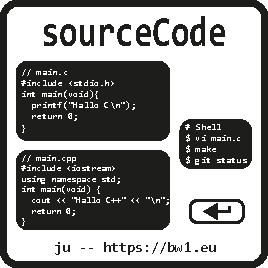
\includegraphics[width=1cm]{content/logo-black.pdf}}

	\vspace*{4\baselineskip}
	{\usekomafont{subject}\typ}\par
	

	{\usekomafont{title}\titel\par}
	\vspace*{\baselineskip}
	{\usekomafont{subtitle}\untertitel}\par

	\vfill

\end{titlepage}

\fi
	\ifisbook\cleardoubleemptypage\fi

	% (Haupt-)Titelseite, Zusammenfassung, ggf. Danksagung & Inhaltsverzeichnis
	\pagenumbering{roman}
	% ju -- https://bw1.eu -- 25-April-18  -- titelpage.tex 
% Modified source from 
% <https://www.dcl.hpi.uni-potsdam.de/media/theses/>
%
\begin{titlepage}
	\setlength{\evensidemargin}{0.5\evensidemargin+0.5\oddsidemargin}
	\setlength{\oddsidemargin}{\evensidemargin}

	\centering
	
	\raisebox{-0.5\height}{
\includegraphics[width=9cm]{content/titelbild.pdf}}
	\hspace*{.2\textwidth}
	\raisebox{-0.5\height}{\includegraphics[width=1cm]{content/logo.pdf}}
	\hfill
	\vspace{3mm}
	{\color{meinblue} \rule{\textwidth}{3pt}}
	

	\vspace*{4\baselineskip}
	{\usekomafont{subject}\typ}\par
	
	\vfill
	{\usekomafont{title}\titel\par}
	\vspace*{\baselineskip}
	{\usekomafont{subtitle}\untertitel}\par
	
	\vfill
	{\textbf{\iflanguage{ngerman}{von}{by}}\\ 
		\smallskip\usekomafont{author}\autor}\par
	
	\vfill
	{\usekomafont{date}\ort}\par

	\vspace*{\baselineskip}
	{\usekomafont{date}\datum}\par
  
	\begin{flushleft}
	\vfill
  {\qrcode[hyperlink,height=1.5cm]{\website}}\par
	\end{flushleft}

	\setcounter{page}{1}

\end{titlepage}


	\ifisbook\cleardoubleemptypage\fi% ju -- https://bw1.eu -- 25-April-18  -- zusammenfassung.tex 
% Modified source from 
% <https://www.dcl.hpi.uni-potsdam.de/media/theses/>
%
% deutsche Zusammenfassung
\null\vfil
\begin{otherlanguage}{ngerman}
\begin{center}\textsf{\textbf{\abstractname}}\end{center}

\noindent Dies hier ist ein Blindtext zum Testen von Textausgaben. Wer diesen Text liest, 
ist selbst schuld. Der Text gibt lediglich den Grauwert der Schrift an. 
Ist das wirklich so? Ist es gleichgültig, ob ich schreibe: "Dies ist ein Blindtext" 
oder "Huardest gefburn"? Kjift - mitnichten! Ein Blindtext bietet mir wichtige Informationen.

\end{otherlanguage}
\vfil\null



% example
	\ifisbook\cleardoubleemptypage\fi% ju -- https://bw1.eu -- 25-April-18  -- danksagung.tex 
% Modified source from 
% <https://www.dcl.hpi.uni-potsdam.de/media/theses/>
%
\vspace*{\fill}
\begin{center}\textsf{\textbf{Danksagung}}\end{center}

\noindent Dies hier ist ein Blindtext zum Testen von Textausgaben. Wer diesen Text liest, 
ist selbst schuld. Der Text gibt lediglich den Grauwert der Schrift an. 
Ist das wirklich so? Ist es gleichgültig, ob ich schreibe: "Dies ist ein Blindtext" 
oder "Huardest gefburn"? Kjift - mitnichten! Ein Blindtext bietet mir wichtige Informationen.

\vspace*{\fill}% example
	\tableofcontents
	\cleardoublepage

	% Textteil
	\pagenumbering{arabic}
	

	% Inhalt 
% ju -- https://bw1.eu -- 26-Okt-18
\chapter{Kapitel} 
\input{tex/1-Readme}

\chapter{Kapitel} 
\input{tex/7-gitWorkflow}

\chapter{Kapitel} 
\input{tex/RasperryPi}

 % wird per Powershell Script ersetzt
  
  \chapter{Kapitel}
	% ju -- https://bw1.eu -- 25-April-18  -- kap1.tex 
%\chapter{Kapitel}
%
\section{\LaTeX - Spickzettel}\label{sec:LaTeX-Spickzettel}

\subsection{Blindtext}\label{sec:blindtext}

\blindtext[1] 

\blindtext[1]

\subsection{Flattersatz versus Blocksatz}\label{sec:Flattersatz-versus-Blocksatz}

\begin{flushleft}
\blindtext[1]
\end{flushleft}

\begin{flushright}
\blindtext[1]
\end{flushright}

\begin{center}
\blindtext[1]
\end{center}

\newpage

\subsection{Gliederung}

% Quellcode Referenz
(\autoref{code:gliederung} Gliederung).
% Quellcode
\lstset{language=[LaTeX]TeX} % C, [LaTeX]TeX, Bash, Python
\begin{lstlisting}[columns=fullflexible,%numbers=left, frame=l, framerule=0.1pt,%
% ======================
  caption={Gliederung},    % Caption anpassen!
  label={code:gliederung}  % Label anpassen!
]% ======================

	% artikel:         Textabstand
	\subsection \subsubsection \paragraph \subparagraph

	% report:
	\chapter \subsection \subsubsection \paragraph \subparagraph

	% * keine Nummerierung
	\subsection*{eins}

	% Sprungmarke
	\label{sec:eins}
\end{lstlisting}

\newpage

\subsection{Quellcode}

Quellcode \verb|Code|.

% Quellcode Referenz
(\autoref{code:dummyCode} dummyCode).  % Anpassen!
% Quellcode
\lstset{language=[LaTeX]TeX} % C, [LaTeX]TeX, Bash, Python
\begin{lstlisting}[columns=fullflexible,%numbers=left, frame=l, framerule=0.1pt,%
% ======================
  caption={dummyCode},    % Caption anpassen!
  label={code:dummyCode}  % Label anpassen!
]% ======================

	/* Quellcode */
\end{lstlisting}

% Quellcode Ausgabe Referenz
(\autoref{code:dummyCode-out} dummyCode Ausgabe).  % Anpassen!
% Quellcode
\lstset{language=[LaTeX]TeX} % C, [LaTeX]TeX, Bash, Python
\begin{lstlisting}[columns=fullflexible,%numbers=left, frame=l, framerule=0.1pt,%
% ======================
  caption={dummyCode Ausgabe},    % Caption anpassen!
  label={code:dummyCode-out}  % Label anpassen!
]% ======================

	% Quellcode Referenz
	(\autoref{code:dummyCode} dummyCode).  % Anpassen!
	% Quellcode
	\lstset{language=[LaTeX]TeX} % C, [LaTeX]TeX, Bash, Python
	\begin{lstlisting}[columns=fullflexible,%numbers=left, frame=l, framerule=0.1pt,%
	% ======================
		caption={dummyCode},    % Caption anpassen!
		label={code:dummyCode}  % Label anpassen!
	]% ======================

		/* Quellcode */
	%end{lstlisting}
\end{lstlisting}

% Quellcode Referenz
(\autoref{code:hallo-ext} hallo.c).    % codename = 
% Quellcode aus ext. Datei
	\lstset{language=C}% C++, [LaTeX]TeX, Bash, Python
	\lstinputlisting[%numbers=left, frame=l, framerule=0.1pt,
	% =====================
	caption={Quellcode in C, hallo.c},    % Caption  anpassen!
	label={code:hallo-ext}  % Referenz anpassen!
	% =====================
	]{content/hallo.c}% ext. Datei

\newpage

\subsection{Querverweise-Referenzen}\label{sec:quer-ref}

(\autoref{sec:schriftstile} Schriftstile).

(\autoref{sec:listen} Listen).

(\autoref{pic:tux1} Tux1).

\begin{enumerate}
	\item zuerst
	\item \label{item:folge} folgend
	\item abschließend
\end{enumerate}

Wir verweisen auf ein Listenelement \autoref{item:folge}.

% Quellcode Ausgabe Referenz
(\autoref{code:quer-ref-out} Querverweise-Referenzen).% Anpassen!
% Quellcode
\lstset{language=[LaTeX]TeX} % C, [LaTeX]TeX, Bash, Python
\begin{lstlisting}[columns=fullflexible,%numbers=left, frame=l, framerule=0.1pt,%
% ======================
	caption={Quellcode in LaTeX, Querverweise-Referenzen},% Anpassen!
	label={code:quer-ref-out}%
	%============================
]
	(\autoref{sec:schriftstile} Schriftstile).
	(\autoref{sec:listen} Listen).
	(\autoref{pic:tux1} Tux1).
	\begin{enumerate}
		\item zuerst
		\item \label{item:folge} folgend
		\item abschließend
	\end{enumerate}
	Wir verweisen auf ein Listenelement \autoref{item:folge}.
\end{lstlisting}

% Tabelle Referenz
(\autoref{tab:label-verweis} Label Querverweis).
% Tabelle
\begin{table}[!hb] % hier einfügen
	%============================
	\caption{Label Querverweis }	% Caption anpassen!
  \label{tab:label-verweis}	% Referenz anpassen!
	%============================
	\centering
	\begin{tabular} {ll}
	\toprule % Inhalt
		Abk. & Beschreibung \\
  \midrule
		sec  & für alle Gliederungsebenen \\
		cha  & oder chap für Kapitel (es kann aber auch sec verwendet werden) \\
		part & für Teile eines Buches (ebenso sec möglich) \\
		fig  & für Abbildungen \\
		tab  & für Tabellen \\
		item & für Aufzählungspunkte \\
		eqn  & für Gleichungen  \\
		fn   & für Fußnoten \\
		code & Listing \\
		pic  & Grafik \\
	\bottomrule
	\end{tabular}
\end{table}

\newpage

\subsection{Zitieren}\label{sec:zitieren}

\begin{quote}
Ein schönes Zitat von einem schlauen Menschen steht den meisten Dokumenten
gut zu Gesicht.
\end{quote}

Fussnote\footnote{Fussnote}.

Google\footnote{\url{https://www.google.de/}}

Anfang ">Anführungszeichen."< Ende

Anfang "`Anführungszeichen."' Ende

Anfang \flqq Anführungszeichen.\frqq Ende

\LaTeX buch \cite{Schlosser201609}.

% Quellcode Referenz
(\autoref{code:zitieren-out} Zitieren).
% Quellcode
\lstset{language=[LaTeX]TeX} % C, [LaTeX]TeX, Bash, Python
\begin{lstlisting}[columns=fullflexible,%numbers=left, frame=l, framerule=0.1pt,%
% ======================
	caption={Quellcode in LaTeX, Zitieren},% Anpassen!
	label={code:zitieren-out}%
	%============================
]
	\begin{quote}
		Ein schönes Zitat von einem schlauen Menschen steht 
		den meisten Dokumenten gut zu Gesicht.
	\end{quote}
	Fussnote\footnote{Fussnote}.
	Anfang ">Anführungszeichen."< Ende
	Anfang "`Anführungszeichen."' Ende
	Anfang \flqq Anführungszeichen.\frqq Ende
	\LaTeX buch \cite{Schlosser201609}.
\end{lstlisting}

\newpage

\subsection{Links}\label{sec:links}\index{Links}

Darstellung einer klickbaren URL: \url{https://www.google.de/}

Text, der auf eine Webseite linkt: \href{https://bw1.eu/}{Meine Webseite}

Emailadresse verlinken: \href{mailto:info@bw1.eu}{Meine E-Mail-Adresse}

auf lokale Datei verlinken: \href{run:/word.docx}{lokale Datei} 

PDF einbinden: 
\includepdf[pagecommand={\thispagestyle{headings}},
	noautoscale=true,width=0.9\textwidth,offset=0cm -1cm]{content/titelbild.pdf}

PDF einbinden: \\ 


\includegraphics[width=0.9\textwidth]{content/titelbild.pdf}


(\autoref{code:links-out} Links).
% Quellcode
\lstset{language=[LaTeX]TeX} % C, [LaTeX]TeX, Bash, Python
\begin{lstlisting}[columns=fullflexible,%numbers=left, frame=l, framerule=0.1pt,%
% ======================
	caption={Quellcode in LaTeX, Links},% Anpassen!
	label={code:links-out}%
	%============================
]
	Darstellung einer klickbaren URL: \url{https://www.google.de/}

	Text, der auf eine Webseite linkt: \href{https://bw1.eu/}{Meine Webseite}

	Emailadresse verlinken: \href{mailto:info@bw1.eu}{Meine E-Mail-Adresse}

	auf lokale Datei verlinken: \href{run:/word.docx}{lokale Datei} 

	PDF einbinden: 
\includepdf[pagecommand={\thispagestyle{headings}},
		noautoscale=true,width=0.9\textwidth,offset=0cm -1cm]{content/titelbild.pdf}

	PDF einbinden: \\
	
	
\includegraphics[width=0.9\textwidth]{content/titelbild.pdf}
\end{lstlisting}

\newpage

\subsection{Farbe}

Text \textcolor{red}{rot} Text

Text \colorbox{hellesbrombeer}{hellesbrombeer} Text

\colorbox{red!10!white}{10 \% rot, Rest weiß}

\textcolor{meinorange}{farbiger Text}
\textcolor{meinblue}{farbiger Text}
\textcolor{meinred}{farbiger Text}
\textcolor{magenta}{farbiger Text}

\wichtig[meinblue]{wichtiger farbiger Text}
\wichtig[meinred]{wichtiger farbiger Text}
\wichtig[meinorange]{wichtiger farbiger Text}
\wichtig[magenta]{wichtiger farbiger Text}

% Farbbox
\colorbox{meingrey}{Text}
\colorbox{meinorange}{Text}

% bunter Rahmen um eine Formel
\fcolorbox{meinblue}{meingrey}{$a^{2} + b^{2} = c^{2}$}

% Quellcode Referenz
(\autoref{code:farbe-out} Farbe).
% Quellcode
\lstset{language=[LaTeX]TeX} % C, [LaTeX]TeX, Bash, Python
\begin{lstlisting}[columns=fullflexible,%numbers=left, frame=l, framerule=0.1pt,%
% ======================
	caption={Quellcode in LaTeX, Farbe},% Anpassen!
	label={code:farbe-out}%
	%============================
]
	\textcolor{meingreen}{farbiger Text}
	\textcolor{meinblue}{farbiger Text}
	\textcolor{meinred}{farbiger Text}

	\wichtig[meinblue]{wichtiger farbiger Text}
	\wichtig[meinred]{wichtiger farbiger Text}
	\wichtig[meingreen]{wichtiger farbiger Text}

	% Farbbox
	\colorbox{meingrey}{Text}
	\colorbox{meinorange}{Text}

	% bunter Rahmen um eine Formel
	\fcolorbox{meinblue}{meingrey}{$a^{2} + b^{2} = c^{2}$}
\end{lstlisting}

\begin{hinweis}
 Es gibt zwei Möglichkeiten.
 Du schreibst eine for-Schleife, die alle Namen durchgeht und
 abbricht (mit break), wenn ein Name mit D gefunden wurde.
 Du schreibst eine while-Schleife, die der Reihe nach die Namen anschaut,
 solange sie nicht mit D anfangen. Dazu verwendest Du einen Zähler,
 der bei 0 anfängt, und der Reihe nach alle Namen abfragt.
\end{hinweis}

\myInfoBox{
 Es gibt zwei Möglichkeiten.
 Du schreibst eine for-Schleife, die alle Namen durchgeht und
 abbricht (mit break), wenn ein Name mit D gefunden wurde.
 Du schreibst eine while-Schleife, die der Reihe nach die Namen anschaut,
 solange sie nicht mit D anfangen. Dazu verwendest Du einen Zähler,
 der bei 0 anfängt, und der Reihe nach alle Namen abfragt.
}

% Quellcode Referenz
(\autoref{code:hinweis-infobox-out} Hinweis, Infobox).
% Quellcode
\lstset{language=[LaTeX]TeX} % C, [LaTeX]TeX, Bash, Python
\begin{lstlisting}[columns=fullflexible,%numbers=left, frame=l, framerule=0.1pt,%
% ======================
	caption={Quellcode in LaTeX, Hinweis, Infobox},% Anpassen!
	label={code:hinweis-infobox-out}%
	%============================
]
	\begin{hinweis}
	 Es gibt zwei Möglichkeiten.
	 Du schreibst eine for-Schleife, die alle Namen durchgeht und
	 abbricht (mit break), wenn ein Name mit D gefunden wurde.
	 Du schreibst eine while-Schleife, die der Reihe nach die Namen anschaut,
	 solange sie nicht mit D anfangen. Dazu verwendest Du einen Zähler,
	 der bei 0 anfängt, und der Reihe nach alle Namen abfragt.
	\end{hinweis}

	\myInfoBox{
	 Es gibt zwei Möglichkeiten.
	 Du schreibst eine for-Schleife, die alle Namen durchgeht und
	 abbricht (mit break), wenn ein Name mit D gefunden wurde.
	 Du schreibst eine while-Schleife, die der Reihe nach die Namen anschaut,
	 solange sie nicht mit D anfangen. Dazu verwendest Du einen Zähler,
	 der bei 0 anfängt, und der Reihe nach alle Namen abfragt.
	}
\end{lstlisting}

\newpage

\subsection{Tabellen}\label{sec:tabellen}

\begin{tabular}{ccc}
	\toprule
		Leistung & 45 & kWh \\
	\midrule
		Hubraum & $1234$ & $cm^3$ \\
		Preis & 23499 & Euro \\
	\bottomrule
\end{tabular}\\

Text

% Tabellen Referenz
(\autoref{tab:dummyTabelle} dummyTabelle).
% Tabelle
\begin{table}[!hb] % hier
	\centering
	%\setlength{\tabcolsep}{5mm}      % Spaltenlänge fest
	%\begin{tabularx}{\textwidth}{XX} % auto. Spaltenumbruch
	\rowcolors{1}{ }{lightgray!20} % Farbe
	\begin{tabular} {ll}
		\toprule 
		%\rowcolor{orange!90} % Farbe
		%============================
	  \textbf{A} & \textbf{B} \\
	  \midrule
    a1 & a2 \\
    b1 & b2 \\
    c1 & c2 \\
		%============================
		\bottomrule
	%\end{tabularx}
	\end{tabular}
	%============================
	\caption{dummyTabelle}   % Caption anpassen!
	\label{tab:dummyTabelle} % Referenz anpassen!
	%============================
\end{table}

% Quellcode Referenz
(\autoref{code:dummyTabelle-out} dummyTabelle).
% Quellcode
\lstset{language=[LaTeX]TeX} % C, [LaTeX]TeX, Bash, Python
\begin{lstlisting}[columns=fullflexible,%numbers=left, frame=l, framerule=0.1pt,%
% ======================
	caption={Quellcode in LaTeX, dummyTabelle},% Anpassen!
	label={code:dummyTabelle-out}%
	%============================
]
	% Tabellen Referenz
	(\autoref{tab:dummyTabelle} dummyTabelle).
	% Tabelle
	\begin{table}[!hb] % hier
		\centering
		%\setlength{\tabcolsep}{5mm}% Spaltenlänge fest
		\rowcolors{1}{ }{lightgray!20} % Farbe
		%\begin{tabularx}{\textwidth}{XX}% auto. Spaltenumbruch
		\begin{tabular} {ll}
			\toprule 
			%\rowcolor{meinblue!90}% Farbe
			%============================
				\textbf{A} & \textbf{B} \\
			\midrule
				a1 & a2 \\
				b1 & b2 \\
				c1 & c2 \\
			%============================
			\bottomrule
		%\end{tabularx}
		\end{tabular}
		%============================
		\caption{dummyTabelle}% Caption anpassen!
		\label{tab:dummyTabelle}					  % Referenz anpassen!
		%============================
	\end{table}
\end{lstlisting}

% Tabellen Referenz
(\autoref{tab:spalte-fest} Spaltenlänge fest).
% Tabelle
\begin{table}[!hb] % hier
	\centering
	\setlength{\tabcolsep}{5mm}% Spaltenlänge fest
	%\begin{tabularx}{\textwidth}{XX}% auto. Spaltenumbruch
	\rowcolors{1}{ }{lightgray!20} % Farbe 
	\begin{tabular} {ll}
		\toprule 
		%\rowcolor{meinblue!90}% Farbe
		%============================
	    \textbf{A} & \textbf{B} \\
	  \midrule
			a1 & a2 \\
			b1 & b2 \\
			c1 & c2 \\
		%============================
		\bottomrule
	%\end{tabularx}
	\end{tabular}
	%============================
	\caption{Spaltenlänge fest}% Caption anpassen!
	\label{tab:spalte-fest}					  % Referenz anpassen!
	%============================
\end{table}

(Tabelle Longtable).
% Longtable
\rowcolors{1}{ }{lightgray!20} % Farbe
\begin{longtable}{ll}% Spaltenanzahl, l,r,c,p,X
	\toprule
	%\rowcolor{meinblue!90}% Farbe
	\textbf{A} & \textbf{B} \\
	\midrule
	\endfirsthead
	\toprule
	% Tab.-Fortsetzung
	%\rowcolor{meinblue!90}% Farbe
	\textbf{A} & \textbf{B} \\
	\midrule
	\endhead
	% Inhalt
	a1 & a2 \\
	b1 & b2 \\
	c1 & c2 \\
	a1 & a2 \\
	b1 & b2 \\
	c1 & c2 \\
	a1 & a2 \\
	b1 & b2 \\
	c1 & c2 \\
	a1 & a2 \\
	b1 & b2 \\
	c1 & c2 \\
	c1 & c2 \\
	a1 & a2 \\
	b1 & b2 \\
	c1 & c2 \\
	\bottomrule
\end{longtable}

\newpage

\subsection{Abbildungen}\label{sec:abbildungen}

% Bild Referenz
(\autoref{pic:tux1} Linux Pinguin Tux).
% Bild
\begin{figure}[!hb] % hier
	\centering
  \includegraphics[width=0.3\textwidth]{img/logo.pdf}
	% ====================
	\caption[Tux]{">Ein wohlgenährter, glücklicher, rundlicher Pinguin, ist das
									offizielle Maskottchen des freien Betriebssystemkerns Linux."<
	\newline {(Quelle:~Wikipedia)}}% Caption  anpassen!
	\label{pic:tux1}% Referenz anpassen!
	% ===================
\end{figure}

\includegraphics[height=2cm,width=3cm]{img/logo.pdf}
\includegraphics[angle=45, scale=.2]{img/logo.pdf}

% Bild Referenz
(\autoref{pic:dummyAbb} dummyAbb).    % Anpassen!
% Bild
\begin{figure}[!hb]% hier
	\centering
  \includegraphics[width=0.3\textwidth]{img/logo.pdf}
	% ====================
	\caption{dummyAbb}% Caption  anpassen!
	\label{pic:dummyAbb}% Referenz anpassen!
	% ===================
\end{figure}

% Bild Referenz
(\autoref{pic:bildDrehen} Drehen um 45 Grad).    % Anpassen!
% Bild
\begin{figure}[!hb]% hier
	\centering
  \includegraphics[angle=45,width=0.3\textwidth]{img/logo.pdf}
	% ====================
	\caption{Drehen um 45 Grad}% Caption  anpassen!
	\label{pic:bildDrehen}% Referenz anpassen!
	% ===================
\end{figure}

\newpage


% Quellcode Referenz
(\autoref{code:dummyAbb-out} dummyAbb).
% Quellcode
\lstset{language=[LaTeX]TeX} % C, [LaTeX]TeX, Bash, Python
\begin{lstlisting}[columns=fullflexible,%numbers=left, frame=l, framerule=0.1pt,%
% ======================
	caption={Quellcode in LaTeX, dummyAbb},% Anpassen!
	label={code:dummyAbb-out}%
	%============================
]
	% Bild Referenz
	(\autoref{pic:dummyAbb} dummyAbb).    % Anpassen!
	% Bild
	\begin{figure}[!hb]% hier
		\centering
		\includegraphics[width=0.3\textwidth]{img/logo.pdf}
		% ====================
		\caption{dummyAbb}% Caption  anpassen!
		\label{pic:dummyAbb}% Referenz anpassen!
		% ===================
	\end{figure}
\end{lstlisting}

\newpage

\subsection{Scalieren}\index{Skalieren}

Inhalt n-fach scalieren

\vspace{10mm}

\scalebox{3}{Text}
\scalebox{4}{Text}
\scalebox{5}{Text}

\subsection{Rotieren}

Inhalt rotieren - Wert in Grad

\vspace{10mm}

\rotatebox{45}{Text}
\rotatebox{90}{Text}
\rotatebox{180}{Text}


% Quellcode Referenz
(\autoref{code:scal-rot-out} Scalieren und Rotieren).
% Quellcode
\lstset{language=[LaTeX]TeX} % C, [LaTeX]TeX, Bash, Python
\begin{lstlisting}[columns=fullflexible,%numbers=left, frame=l, framerule=0.1pt,%
% ======================
	caption={Quellcode in LaTeX, Scalieren und Rotieren},% Anpassen!
	label={code:scal-rot-out}%
%============================
]
	% Inhalt n-fach scalieren
	\scalebox{3}{Text}
	\scalebox{4}{Text}
	\scalebox{5}{Text}

	% Inhalt rotieren - Wert in Grad
	\rotatebox{45}{Text}
	\rotatebox{90}{Text}
	\rotatebox{180}{Text}
\end{lstlisting}

\newpage

\subsection{Gliederung in Kapitel und Abschnitte}\label{sec:Gliederung-Kapitel-Abschnitte}

(\autoref{tab:Gliederung-Kapitel-Abschnitte} Gliederung in Kapitel und Abschnitte).
% Tabelle
\begin{table}[!hb]% hier 
	\centering
	%\setlength{\tabcolsep}{5mm}% Spaltenlänge fest
  \rowcolors{1}{ }{lightgray!20} % Farbe
	%\begin{tabularx}{\textwidth}{XX}% auto. Spaltenumbruch
	\begin{tabular} {ll}
		\toprule % Inhalt
		%\rowcolor{meinblue!90}% Farbe
		%============================
		\verb|#| & \textbf{Beschreibung} \\
	  \midrule
		\verb|\chapter{}      | & Ein Kapitel\\
		\verb|\section{}      | & Ein Abschnitt\\
		\verb|\subsection{}   | & Ein Unterabschnitt\\
		\verb|\subsubsection{}| & Ein Unter-Unterabschnitt\\
		\verb|\paragraph{}    | & Ein Absatz\\
		\verb|\subparagraph{} | & Ein Unterabsatz\\
		\verb|\subsection*{}  | & Ein unnummerierter Abschnitt\\
		\verb|\subsection[Kurzer Titel]{}| & langer Abschnittstitel\\
		%============================
		\bottomrule
	%\end{tabularx}
	\end{tabular}
	\caption{Gliederung in Kapitel und Abschnitte}	% Caption anpassen!
	\label{tab:Gliederung-Kapitel-Abschnitte}	% Referenz anpassen!
	%============================
\end{table}

\subsection{Schriftstile}\label{sec:schriftstile}

\emph{kursiv}
\textrm{Antiqua}, \textsf{Grotesk}, \texttt{Maschinenschrift},
\textmd{normal}, \textbf{breiter}, \textup{aufrecht}, \textsl{geneigt},
\textit{kursiv}, \textsc{Kapitaelchen}

\subsection{Schriftgrößen}

\tiny{winzig}, \scriptsize{sehr klein}, \footnotesize{klein},
\small{klein}, , \large{gross}, \Large{groesser},
\LARGE{ganz gross}, \huge{riesig}, \Huge{gigantisch} \normalsize{normal}

\subsection{Wortabstände}\label{sec:Wortabstaende}

(\autoref{tab:wortabstand} Wortabstände).
% Tabelle
\begin{table}[!hb] % hier 
	\centering
	%\setlength{\tabcolsep}{5mm}% Spaltenlänge fest
	\rowcolors{1}{ }{lightgray!20} % Farbe
	%\begin{tabularx}{\textwidth}{XX}% auto. Spaltenumbruch
	\begin{tabular} {ll}
	\toprule % Inhalt
	%\rowcolor{meinblue!90}% Farbe
	%============================
	\verb|#| & \textbf{Beschreibung} \\
	\midrule
			\verb|\| & erzeugt Leerstelle \\
			\verb|\@| & kennzeichnet einen Punkt als Satzende \\
			\verb|~| & erzeugt nicht umbrechbare Leerstelle \\
			\verb|\,| & erzeugt nicht umbrechbare Leerstelle \\
			\verb|\quad| & erzeugt einfach vergrößerten Abstand \\
			\verb|\qquad| & erzeugt vierfach vergrößerten Abstand \\
			\verb|\hspace{1cm}| & erzeugt Abstand von 1cm Breite \\
			\verb|\hfill| & fügt so viel Leerraum ein wie möglich \\
			\verb|\smallskip| & vertikaler Abstand\\
			\verb|\medskip| & \\
			\verb|\bigskip| & \\
			\verb|\vspace{1cm}| & \\
			\verb|\vfill| & \\
	%============================
	\bottomrule
	%\end{tabularx}
	\end{tabular}
	\caption{Wortabstände }	% Caption anpassen!
	\label{tab:wortabstand}	% Referenz anpassen!
	%============================
\end{table}

\subsection{Logische Textauszeichnung}\label{sec:LogischeTextauszeichnung}

(\autoref{tab:Textauszeichnung} Logische Textauszeichnung).
% Tabelle
\begin{table}[!hb] % hier 
	\centering
	%\setlength{\tabcolsep}{5mm}% Spaltenlänge fest
	\rowcolors{1}{ }{lightgray!20} % Farbe
	%\begin{tabularx}{\textwidth}{XX}% auto. Spaltenumbruch
	\begin{tabular} {ll}
	\toprule % Inhalt
	%\rowcolor{meinblue!90}% Farbe
	%============================
	\verb|#| & \textbf{Beschreibung} \\
	\midrule
			\verb|\emph{Hervorhebung}| & \emph{Hervorhebung} \\
			 \verb|\url{http://www.dante.de/}| & \url{http://www.dante.de/} \\
			 \verb|\href{https://bw1.eu/}{Meine Webseite} |& \href{https://bw1.eu/}{Meine Webseite} \\
			 \verb|\href{mailto:info@bw1.eu}{info@bw1.eu} |& \href{mailto:info@bw1.eu}{info@bw1.eu} \\
			 \verb|\path{/home/foo/meindok.tex}| & \path{/home/foo/meindok.tex} \\
			 \verb|\path{C:\TEMP\meindok.tex}| & \path{C:\TEMP\meindok.tex} \\
			 \verb|\wort{Text} | & \wort{Text} \\
			 \verb|\fremdwort{Text} |& \fremdwort{Text} \\
			 \verb|Sonderzeichen: \& \% \$ \# \_ \{ \} |& \& \% \$ \# \_ \{ \} \\
			 \verb|\LaTeX|& \LaTeX \\
			 \verb|\dots|& \dots \\
	%============================
	\bottomrule
	%\end{tabularx}
	\end{tabular}
	\caption{Logische Textauszeichnung}	% Caption anpassen!
	\label{tab:Textauszeichnung}	% Referenz anpassen!
	%============================
\end{table}

\subsection{Punkte}\label{sec:Punkte}

(\autoref{tab:punkt} Punkte).
% Tabelle
\begin{table}[!hb] % hier einfügen
	\centering
	%\setlength{\tabcolsep}{5mm}% Spaltenlänge fest
	\rowcolors{1}{ }{lightgray!20} % Farbe
	%\begin{tabularx}{\textwidth}{XX}% auto. Spaltenumbruch
	\begin{tabular} {ll}
	\toprule % Inhalt
	%\rowcolor{meinblue!90}% Farbe
	%============================
	\verb|#| & \textbf{Beschreibung} \\
	\midrule
	\verb|Deutsch: Eins, zwei, ...| & Deutsch: Eins, zwei, ... \\
	\verb|Amerikanisch: One, two,~\dots| & Amerikanisch: One, two,~\dots \\
	%============================
	\bottomrule
	%\end{tabularx}
	\end{tabular}
	\caption{Punkte }	% Caption anpassen!
	\label{tab:punkt}	% Referenz anpassen!
	%===========================
\end{table}

\subsection{Binde- und Gedankenstriche}\label{sec:Binde-Gedankenstriche}

(\autoref{tab:Bindestriche } Binde- und Gedankenstriche).
% Tabelle
\begin{table}[!hb]% hier 
	\centering
	%\setlength{\tabcolsep}{5mm}% Spaltenlänge fest
	\rowcolors{1}{ }{lightgray!20} % Farbe
	%\begin{tabularx}{\textwidth}{XX}% auto. Spaltenumbruch
	\begin{tabular} {ll}
	\toprule % Inhalt
	%\rowcolor{meinblue!90}% Farbe
	%============================	
	\verb|#| & \textbf{Beschreibung} \\
	\midrule
	\verb|n-zu-m-Abbildung| & n-zu-m-Abbildung \\
	\verb|11--19 Uhr| & 11--19 Uhr \\
	\verb|Berlin--Hamburg| & Berlin--Hamburg \\
	\verb|wahr -- oder falsch?| & wahr -- oder falsch? \\
	\verb|true---or false?| & true---or false? \\
	\verb|1, 0, $-$| & 1, 0, $-$ \\
	%============================
	\bottomrule
	%\end{tabularx}
	\end{tabular}
	\caption{Binde- und Gedankenstriche }	% Caption anpassen!
	\label{tab:Bindestriche }	% Referenz anpassen!
	%===========================
\end{table}

\newpage

\subsection{Listen}\label{sec:listen}

%% Liste
\begin{itemize}% Liste Punkt
	\item Text
	\item Text
\end{itemize}

\begin{enumerate}% Liste Aufzählung
	\item Text
	\item Text
\end{enumerate}

\begin{enumerate}% Liste 1.
	\item Text
	\begin{enumerate}% Liste a)
		\item Text
		\item Text
	\end{enumerate}% Liste 2.
	\item Text
	\begin{enumerate}% Liste b)
		\item Text
		\item Text
	\end{enumerate}
\end{enumerate}

\begin{enumerate}[label=(\roman*)]% (i), (ii), (iii) ...
	\item Text
	\item Text
\end{enumerate}

\begin{enumerate}[label={\arabic*\alph*)}]% 1a), 2b), 3c) ...
	\item Text
	\item Text
\end{enumerate}

\begin{enumerate}[label=\bfseries Punkt \Roman*]% Punkt I, Punkt II, Punkt III ...
	\item Text
	\item Text
\end{enumerate}

\section{Mathe - Beispiele}\label{mathe-bsp}

% \begin{align}	\quad \text{;} \quad \end{align}

\num{12345,678999}


\subsection{Potenzen }\label{sec:potenzen }\index{Potenzen }

allgemein:

\begin{align}
a^n &= a \cdot a \cdot ... \cdot a_n
\end{align}

Multiplikation: (gl.Basis, gl. Exponent)

\begin{align}
a^n \cdot a^m &= a^{n+m} \\
a^n \cdot b^n &= (a \cdot b)^n
\end{align}

Division:

\begin{align}
\frac{a^n}{a^m} &= a^{n-m} \\
a^{-n}          &= \frac{1}{a^n}   \\
a^0 						&= 1 \\
a^1				      &= a
\end{align}

Potenzen potenzieren:

\begin{align}
(a^n)^m         &= a^{n \cdot m} \\
\frac{a^n}{b^n} &= \left(\frac{a}{b}\right)^n
\end{align}

\begin{align}
a^b        &= e^{b \cdot ln \, a} \\
\sqrt[n]{a^m} &= a^{\frac{m}{n}}
\end{align}

(\autoref{code:mathe-out} Mathe).
% Quellcode
\lstset{language=[LaTeX]TeX} % C, [LaTeX]TeX, Bash, Python
\begin{lstlisting}[columns=fullflexible,%numbers=left, frame=l, framerule=0.1pt,%
% ======================
	caption={Quellcode in LaTeX, Mathe},% Anpassen!
	label={code:mathe-out}%
%============================
]
	allgemein:

	\begin{align}
	a^n &= a \cdot a \cdot ... \cdot a_n
	\end{align}

	Multiplikation: (gl.Basis, gl. Exponent)

	\begin{align}
	a^n \cdot a^m &= a^{n+m} \\
	a^n \cdot b^n &= (a \cdot b)^n
	\end{align}

	Division:

	\begin{align}
	\frac{a^n}{a^m} &= a^{n-m} \\
	a^{-n}          &= \frac{1}{a^n}   \\
	a^0 						&= 1 \\
	a^1				      &= a
	\end{align}

	Potenzen potenzieren:

	\begin{align}
	(a^n)^m         &= a^{n \cdot m} \\
	\frac{a^n}{b^n} &= \left(\frac{a}{b}\right)^n
	\end{align}

	\begin{align}
	a^b        &= e^{b \cdot ln \, a} \\
	\sqrt[n]{a^m} &= a^{\frac{m}{n}}
	\end{align}
\end{lstlisting}

\newpage

\section{LaTeX - Befehle}

Textauszeichnung

(\autoref{code:textauszeichnung-out} Textauszeichnung).
% Quellcode
\lstset{language=[LaTeX]TeX} % C, [LaTeX]TeX, Bash, Python
\begin{lstlisting}[columns=fullflexible,%numbers=left, frame=l, framerule=0.1pt,%
% ======================
	caption={Quellcode in \LaTeX: Textauszeichnung},label={code:textauszeichnung-out}]
	\emph{kursiv}
	\textrm{Antiqua}, \textsf{Grotesk}, \texttt{Maschinenschrift},
	\textmd{normal}, \textbf{breiter}, \textup{aufrecht}, \textsl{geneigt},
	\textit{kursiv}, \textsc{Kapitaelchen}
\end{lstlisting}

Schriftgroesse

(\autoref{code:schriftgroesse-out} Schriftgroesse).
% Quellcode
\lstset{language=[LaTeX]TeX} % C, [LaTeX]TeX, Bash, Python
\begin{lstlisting}[columns=fullflexible,%numbers=left, frame=l, framerule=0.1pt,%
% ======================
	caption={Quellcode in \LaTeX: Schriftgroesse},label={code:schriftgroesse-out}]
  \tiny{winzig}, \scriptsize{sehr klein}, \footnotesize{klein},
	\small{klein}, \normalsize{normal}, \large{gross}, \Large{groesser},
	\LARGE{ganz gross}, \huge{riesig}, \Huge{gigantisch}
\end{lstlisting}

 eigene Befehle definieren

(\autoref{code:eigene-Befehle-definieren-out} eigene Befehle definieren).
% Quellcode
\lstset{language=[LaTeX]TeX} % C, [LaTeX]TeX, Bash, Python
\begin{lstlisting}[columns=fullflexible,%numbers=left, frame=l, framerule=0.1pt,%
% ======================
	caption={Quellcode in \LaTeX: eigene Befehle definieren},label={code:eigene-Befehle-definieren-out}]
	\wort{Beispiel}
	\fremdwort{prezioes}
	\abstand{}

	\newcommand{\wort}[1]{\emph{#1}}
	\newcommand{\fremdwort}[1]{\textsf{#1}}
	\newcommand{\abstand}[1]{\vspace{5mm}{#1}}
	\newcommand{\wichtig}[2][red]{\textcolor{#1}{\emph{#2}}}

	quad, qquad, hspace{20mm}, vspace{20mm}
	Wichtig (Optionale Parameter)
	Wort Kursiv u. in Farbe
\end{lstlisting}

Eigene Umgebung

(\autoref{code:Eigene-Umgebung-out} Eigene Umgebung).
% Quellcode
\lstset{language=[LaTeX]TeX} % C, [LaTeX]TeX, Bash, Python
\begin{lstlisting}[columns=fullflexible,%numbers=left, frame=l, framerule=0.1pt,%
% ======================
	caption={Quellcode in \LaTeX: TEigene Umgebung},label={code:Eigene-Umgebung-out}]
	Verwendung: \begin{hinweis}Ein Text.\end{hinweis}

	\newenvironment{hinweis}[1][Hinweis]{%
	  \begin{quote}
	  \color{meinblue}\rule{0.87\textwidth}{1pt}\\%
		\color{black}
	  \textbf{#1:}\\ %
	}{%
		\vspace{1mm}
	  \\\color{meinblue}\rule[5ex]{0.87\textwidth}{1pt}%
	  \end{quote}
	}
\end{lstlisting}

farbige Infobox

(\autoref{code:farbigeInfobox-out} farbige Infobox).
% Quellcode
\lstset{language=[LaTeX]TeX} % C, [LaTeX]TeX, Bash, Python
\begin{lstlisting}[columns=fullflexible,%numbers=left, frame=l, framerule=0.1pt,%
% ======================
	caption={Quellcode in \LaTeX: farbige Infobox},label={code:farbigeInfobox-out}]
	Anwendung: \myInfoBox{Text}

	\newcommand\myInfoBox[1]{%
	  \begin{quote}
		\fcolorbox{meinblue}{meingrey}{%
			\parbox{0.85\textwidth}{%
				\textbf{Hinweis:}\\%
				#1
			}
		}
	\end{quote}
	}
\end{lstlisting}

farbige Listenbox

(\autoref{code:farbigeListenbox-out} farbige Listenbox).
% Quellcode
\lstset{language=[LaTeX]TeX} % C, [LaTeX]TeX, Bash, Python
\begin{lstlisting}[columns=fullflexible,%numbers=left, frame=l, framerule=0.1pt,%
% ======================
	caption={Quellcode in \LaTeX: farbige Listenbox},label={code:farbigeListenbox-out}]
	Anwendung:
	\myListenBox {
		\item Listenpunkt
		\item Listenpunkt
		\item Listenpunkt
	}

	\newcommand\myListenBox[1]{%
		\begin{quote}
			\fcolorbox{meinblue}{white}{%
				\parbox{0.85\textwidth}{%
					% Inhalt
					\textbf{Liste: }
					\begin{itemize}[label=$\square$]%checkbox
						#1
					\end{itemize}
				}
			}
		\end{quote}
	}
\end{lstlisting}

(\autoref{code:begriffe-out} Begriffe).
% Quellcode
\lstset{language=[LaTeX]TeX} % C, [LaTeX]TeX, Bash, Python
\begin{lstlisting}[columns=fullflexible,%numbers=left, frame=l, framerule=0.1pt,%
% ======================
	caption={Quellcode in \LaTeX: Begriffe},label={code:begriffe-out}]
	Referenz: 				siehe~\ref{sec:abschnitt}.
	Zitat: 						siehe~\cite{Bos15}.
	Textauszeichnung: \wort{Beispiel}, \fremdwort{Fremdwort}
	Textabstand: 			\abstand{}
	Zahl Einheit: 		1\,l   z.\,B.
	nicht trennpaares Leerzeichen: ~
	Sonderzeichen: 		\& \% \$ \%
	Webadresse:				\url{http://www.LaTeXbuch.de}

	twoside=true		mschaltung Zweiseitig/Einseitiges Layout
	fontsize=12pt		Schriftgröße
	BCOR=10mm			  Bindekorrektur
	parskip					Gibt an wie neue Absätze gekennzeichnet werden.
								Hier empfohlene Beispielwerte:
									false:	Einzug der ersten Zeile
									half:		vertikaler Abstand von einer halben Zeile
									full:		vertikaler Abstand von einer Zeile
	paper=a4				DIN A4 Papier
	toc=listof			Im Inhaltsverzeichnis werden verzeichnisse wie Abbildungsverz.
								aufgenommen, wenn nicht gewünscht toc=nolistof
	toc=bib				  Literaturverzeichnis ohne Nummer im Inhaltsverzeichnis, oder nöchste zeile
	bibliography=totocnumbered	Literaturverzeichnis mit Nummer im Inhaltsverzeichnis, totoc ohne nummer
	open=right			Ein neues Kapitel fängt immer auf einer rechten Seite an, sonst open=any
	numbers=noenddot Nach DUDEN Werden Gliederungsnummern ohne Punkt am Ende gesetzt.
	headinclude			Kopfzeile zählt mit zum Graubereich der Seite
	headlines=2			zweizeilige Kopfzeile
	footexclude			Fußzeile enthält z.B. nur die Seitenzahl zählt deshalb nicht zum Graubereich der Seite
	pagesize=auto		Sorgt dafür, dass das PDF auch die richtige Größe hat
	version=last		welche Version des KOMA-Scripts verwendet werden soll
\end{lstlisting}

\newpage

\section{Quellenangaben}

Quelle \textcite{schlosser_latex:2016}

Quelle Text\footfullcite{schlosser_latex:2016}

Quelle \cite{schlosser_latex:2016}
%============================
%============================
%============================ % LatexSpickzettel.tex
  

	% ggf. Anhang
	\appendix% ju -- https://bw1.eu -- 25-April-18  -- anhang.tex 
% Modified source from 
% <https://www.dcl.hpi.uni-potsdam.de/media/theses/>
%
\chapter{\appendixname}

\section{Eins}
Auch gibt es niemanden, der den Schmerz an sich liebt, sucht oder wünscht, nur, weil er Schmerz ist, es sei denn, es kommt zu zufälligen Umständen, in denen Mühen und Schmerz ihm große Freude bereiten können. Um ein triviales Beispiel zu nehmen, wer von uns unterzieht sich je anstrengender körperlicher Betätigung, außer um Vorteile daraus zu ziehen? Aber wer hat irgend ein Recht, einen Menschen zu tadeln, der die Entscheidung trifft, eine Freude zu genießen, die keine unangenehmen Folgen hat, oder einen, der Schmerz vermeidet, welcher keine daraus resultierende Freude nach sich zieht? Auch gibt es niemanden, der den Schmerz an sich liebt, sucht oder wünscht, nur, weil er Schmerz ist, es sei denn, es kommt zu zufälligen Umständen, in denen Mühen und Schmerz ihm große Freude bereiten können. Um ein triviales Beispiel zu nehmen, wer von uns unterzieht sich je anstrengender körperlicher Betätigung, außer um Vorteile daraus zu ziehen? Aber wer hat irgend ein Recht, einen Menschen zu tadeln, der die Entscheidung trifft, eine Freude zu genießen, die keine unangenehmen Folgen hat, oder einen, der Schmerz vermeidet, welcher keine daraus resultierende Freude nach sich zieht?Auch gibt es niemanden, der den Schmerz an sich liebt, sucht oder wünscht, nur,

\section{Zwei}
Auch gibt es niemanden, der den Schmerz an sich liebt, sucht oder wünscht, nur, weil er Schmerz ist, es sei denn, es kommt zu zufälligen Umständen, in denen Mühen und Schmerz ihm große Freude bereiten können. Um ein triviales Beispiel zu nehmen, wer von uns unterzieht sich je anstrengender körperlicher Betätigung, außer um Vorteile daraus zu ziehen? Aber wer hat irgend ein Recht, einen Menschen zu tadeln, der die Entscheidung trifft, eine Freude zu genießen, die keine unangenehmen Folgen hat, oder einen, der Schmerz vermeidet, welcher keine daraus resultierende Freude nach sich zieht? Auch gibt es niemanden, der den Schmerz an sich liebt, sucht oder wünscht, nur, weil er Schmerz ist, es sei denn, es kommt zu zufälligen Umständen, in denen Mühen und Schmerz ihm große Freude bereiten können. Um ein triviales Beispiel zu nehmen, wer von uns unterzieht sich je anstrengender körperlicher Betätigung, außer um Vorteile daraus zu ziehen? Aber wer hat irgend ein Recht, einen Menschen zu tadeln, der die Entscheidung trifft, eine Freude zu genießen, die keine unangenehmen Folgen hat, oder einen, der Schmerz vermeidet, welcher keine daraus resultierende Freude nach sich zieht?Auch gibt es niemanden, der den Schmerz an sich liebt, sucht oder wünscht, nur,

\section*{Drei (ohne extra Eintrag im Inhaltsverzeichnis)}
Auch gibt es niemanden, der den Schmerz an sich liebt, sucht oder wünscht, nur, weil er Schmerz ist, 

\section*{Vier (ohne extra Eintrag im Inhaltsverzeichnis)}
Auch gibt es niemanden, der den Schmerz an sich liebt, sucht oder wünscht, nur, weil er Schmerz ist,  % example

	% Bibliographie
	\ifisbook\cleardoubleemptypage\fi
	\phantomsection\addcontentsline{toc}{chapter}{\refname}
	\printbibliography[category=cited]

	% Eigenstaendigkeitserklaerung
	\ifisbook\pagestyle{plain}\cleardoubleemptypage% ju -- https://bw1.eu -- 25-April-18  -- erklaerung.tex 
% Modified source from 
% <https://www.dcl.hpi.uni-potsdam.de/media/theses/>
%
\begin{otherlanguage}{ngerman}

\begin{center}\textsf{\textbf{Eidesstattliche Erklärung}}\end{center}
Hiermit versichere ich, dass meine Arbeit \enquote{\titel} selbständig verfasst wurde und dass keine anderen Quellen und Hilfsmittel als die angegebenen benutzt wurden. Diese Aussage trifft auch für alle Implementierungen und Dokumentationen im Rahmen dieses Projektes zu.\\

\noindent
\ort, den \datum,
\vspace{2cm}

\begin{center}
\begin{tabular}{C{6cm}}
\rowcolor{white}
\hline
{\small({\autor})}
\end{tabular}
\end{center}

\end{otherlanguage}


\fi % example

\end{document}
%============================
%============================
%============================